\documentclass{ximera}

\title{HLT Practice}
\begin{document}
\begin{abstract}
    Practice for Horizontal Line Test.
\end{abstract}
\maketitle


\begin{problem}
    Consider the following graph.
    \begin{center}
        \begin{tikzpicture}
                \begin{axis}[
                    axis x line=middle, 
                    axis y line=middle, 
                    minor tick num=1, 
                    x label style={at={(axis description cs:1,0.5)},anchor=south},
                    y label style={at={(axis description cs:0.5,1)},anchor=west},
                    xlabel={$x$}, 
                    ylabel={$y$},
                    xtick={-5,-4,...,6,7}, 
                    ytick={-5,-4,...,5},
                    xmin=-5.5, 
                    xmax=5.5, 
                    ymin=-5.5, 
                    ymax=5.5
                    ]
                \addplot[<->,domain=-5:5, samples=300]{1/3*x^2-4};
                \end{axis}
        \end{tikzpicture}
    \end{center}
    
    Does this graph represent a function?
    \begin{multipleChoice}
        \choice[correct]{Yes.}
        \choice{No.}
    \end{multipleChoice}
    \begin{feedback}
        Remember that the \textit{Vertical} line test tells you if a graph is likely to represent a function.
    \end{feedback}
    
    \begin{problem}
        Is this graph invertible?
        \begin{multipleChoice}
            \choice{Yes}
            \choice[correct]{No}
        \end{multipleChoice}
        \begin{feedback}
            Recall that the \textit{Horizontal} line test tells you if the graph is likely to be invertible.
        \end{feedback}
    \end{problem}
\end{problem}


\begin{problem}
    Consider the following graph.
    \begin{center}
        \begin{tikzpicture}
                \begin{axis}[
                    axis x line=middle, 
                    axis y line=middle, 
                    minor tick num=1, 
                    x label style={at={(axis description cs:1,0.5)},anchor=south},
                    y label style={at={(axis description cs:0.5,1)},anchor=west},
                    xlabel={$x$}, 
                    ylabel={$y$},
                    xtick={-5,-4,...,6,7}, 
                    ytick={-5,-4,...,5},
                    xmin=-5.5, 
                    xmax=5.5, 
                    ymin=-5.5, 
                    ymax=5.5
                    ]
                \addplot[->,domain=-4:5, samples=300]{(x+4)^(1/2)};
                \addplot[->,domain=-4:5, samples=300]{-(x+4)^(1/2)};
                \end{axis}
        \end{tikzpicture}
    \end{center}
    
    Does this graph represent a function?
    \begin{multipleChoice}
        \choice{Yes.}
        \choice[correct]{No.}
    \end{multipleChoice}
    \begin{feedback}
        Remember that the \textit{Vertical} line test tells you if a graph is likely to represent a function.
    \end{feedback}
    
    \begin{problem}
        Is this graph invertible?
        \begin{multipleChoice}
            \choice[correct]{Yes}
            \choice{No}
        \end{multipleChoice}
        \begin{feedback}
            Recall that the \textit{Horizontal} line test tells you if the graph is likely to be invertible.
        \end{feedback}
    \end{problem}
\end{problem}


\begin{problem}
    Consider the following graph.
    \begin{center}
        \begin{tikzpicture}
                \begin{axis}[
                    axis x line=middle, 
                    axis y line=middle, 
                    minor tick num=1, 
                    x label style={at={(axis description cs:1,0.5)},anchor=south},
                    y label style={at={(axis description cs:0.5,1)},anchor=west},
                    xlabel={$x$}, 
                    ylabel={$y$},
                    xtick={-5,-4,...,6,7}, 
                    ytick={-5,-4,...,5},
                    xmin=-5.5, 
                    xmax=5.5, 
                    ymin=-5.5, 
                    ymax=5.5
                    ]
                \addplot[<->,domain=-5:5, samples=300]{1/25*x^3};
                \end{axis}
        \end{tikzpicture}
    \end{center}
    
    Does this graph represent a function?
    \begin{multipleChoice}
        \choice[correct]{Yes.}
        \choice{No.}
    \end{multipleChoice}
    \begin{feedback}
        Remember that the \textit{Vertical} line test tells you if a graph is likely to represent a function.
    \end{feedback}
    
    \begin{problem}
        Is this graph invertible?
        \begin{multipleChoice}
            \choice[correct]{Yes}
            \choice{No}
        \end{multipleChoice}
        \begin{feedback}
            Although this may appear to have a horizontal segment near the origin, it in fact does not. This is a good example of why graphing can be misleading at times.
        \end{feedback}
    \end{problem}
\end{problem}



\begin{problem}
    Consider the following graph.
    \begin{center}
        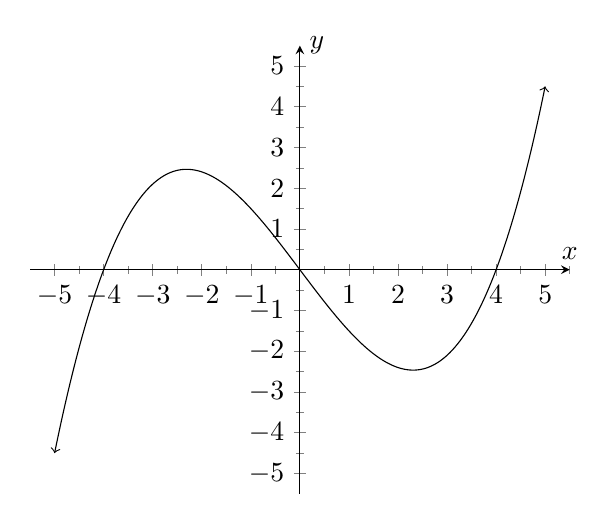
\begin{tikzpicture}
                \begin{axis}[
                    axis x line=middle, 
                    axis y line=middle, 
                    minor tick num=1, 
                    x label style={at={(axis description cs:1,0.5)},anchor=south},
                    y label style={at={(axis description cs:0.5,1)},anchor=west},
                    xlabel={$x$}, 
                    ylabel={$y$},
                    xtick={-5,-4,...,6,7}, 
                    ytick={-5,-4,...,5},
                    xmin=-5.5, 
                    xmax=5.5, 
                    ymin=-5.5, 
                    ymax=5.5
                    ]
                \addplot[<->,domain=-5:5, samples=300]{1/10*x*(x-4)*(x+4)};
                \end{axis}
        \end{tikzpicture}
    \end{center}
    
    Does this graph represent a function?
    \begin{multipleChoice}
        \choice[correct]{Yes.}
        \choice{No.}
    \end{multipleChoice}
    \begin{feedback}
        Remember that the \textit{Vertical} line test tells you if a graph is likely to represent a function.
    \end{feedback}
    
    \begin{problem}
        Is this graph invertible?
        \begin{multipleChoice}
            \choice{Yes}
            \choice[correct]{No}
        \end{multipleChoice}
        \begin{feedback}
            Recall that the \textit{Horizontal} line test tells you if the graph is likely to be invertible.
        \end{feedback}
    \end{problem}
\end{problem}



\begin{problem}
    Consider the following graph.
    \begin{center}
        \begin{tikzpicture}
                \begin{axis}[
                    axis x line=middle, 
                    axis y line=middle, 
                    minor tick num=1, 
                    x label style={at={(axis description cs:1,0.5)},anchor=south},
                    y label style={at={(axis description cs:0.5,1)},anchor=west},
                    xlabel={$x$}, 
                    ylabel={$y$},
                    xtick={-5,-4,...,6,7}, 
                    ytick={-5,-4,...,5},
                    xmin=-5.5, 
                    xmax=5.5, 
                    ymin=-5.5, 
                    ymax=5.5
                    ]
                \addplot[domain=-3:3, samples=300]{(9-x^2)^(1/2)};
                \addplot[domain=-3:3, samples=300]{-(9-x^2)^(1/2)};
                \end{axis}
        \end{tikzpicture}
    \end{center}
    
    Does this graph represent a function?
    \begin{multipleChoice}
        \choice{Yes.}
        \choice[correct]{No.}
    \end{multipleChoice}
    \begin{feedback}
        Remember that the \textit{Vertical} line test tells you if a graph is likely to represent a function.
    \end{feedback}
    
    \begin{problem}
        Is this graph invertible?
        \begin{multipleChoice}
            \choice{Yes}
            \choice[correct]{No}
        \end{multipleChoice}
        \begin{feedback}
            Recall that the \textit{Horizontal} line test tells you if the graph is likely to be invertible.
        \end{feedback}
    \end{problem}
\end{problem}



\begin{problem}
    Consider the following graph.
    \begin{center}
        \begin{tikzpicture}
                \begin{axis}[
                    axis x line=middle, 
                    axis y line=middle, 
                    minor tick num=1, 
                    x label style={at={(axis description cs:1,0.5)},anchor=south},
                    y label style={at={(axis description cs:0.5,1)},anchor=west},
                    xlabel={$x$}, 
                    ylabel={$y$},
                    xtick={-5,-4,...,6,7}, 
                    ytick={-5,-4,...,5},
                    xmin=-5.5, 
                    xmax=5.5, 
                    ymin=-5.5, 
                    ymax=5.5
                    ]
                \addplot[->,domain=0:5, samples=300]{2*x^(1/3)};
                \addplot[<-,domain=-5:0, samples=300]{-2*(-x)^(1/3)};
                \end{axis}
        \end{tikzpicture}
    \end{center}
    
    Does this graph represent a function?
    \begin{multipleChoice}
        \choice[correct]{Yes.}
        \choice{No.}
    \end{multipleChoice}
    \begin{feedback}
        Although this may look like it has a vertical segment right near the origin, it in fact doesn't. This is a good example of why graphing can be a bit misleading at times.
    \end{feedback}
    
    \begin{problem}
        Is this graph invertible?
        \begin{multipleChoice}
            \choice[correct]{Yes}
            \choice{No}
            \begin{feedback}
                Recall that the \textit{Horizontal} line test tells you if the graph is likely to be invertible.
            \end{feedback}
        \end{multipleChoice}
    \end{problem}
\end{problem}




\end{document}